\documentclass[serif, aspectratio=169]{beamer}
\usepackage[T1]{fontenc} 
\usepackage{fourier}
\usepackage{hyperref}
\usepackage{latexsym,amsmath,xcolor,multicol,booktabs,calligra}
\usepackage{booktabs} % For better table formatting
\usepackage{graphicx,pstricks,listings,stackengine}
\usepackage{listings}
\usepackage{array} 
\usepackage{colortbl}

\author{Dr.Hajialiasgari}
\title{Machine Learning}
\institute{
    Tehran University \\
    Of\\
    Medical Science
}
\date{\small \today}
\usepackage{UoWstyle}

% Define custom colors and styles for listings
\definecolor{deepblue}{rgb}{0,0,0.5}
\definecolor{deepred}{RGB}{153,0,0}
\definecolor{deepgreen}{rgb}{0,0.5,0}
\definecolor{halfgray}{gray}{0.55}

\lstset{
    basicstyle=\ttfamily\small,
    keywordstyle=\bfseries\color{deepblue},
    emphstyle=\ttfamily\color{deepred},
    stringstyle=\color{deepgreen},
    numbers=left,
    numberstyle=\small\color{halfgray},
    rulesepcolor=\color{red!20!green!20!blue!20},
    frame=shadowbox,
}

\begin{document}

\begin{frame}
    \titlepage
    \vspace*{-0.6cm}
    \begin{figure}[htpb]
        \begin{center}
            \includegraphics[keepaspectratio, scale=0.05]{Tumsl-logo.png}
        \end{center}
    \end{figure}
\end{frame}

\begin{frame}    
\tableofcontents[sectionstyle=show, subsectionstyle=show/shaded/hide, subsubsectionstyle=show/shaded/hide]
\end{frame}

\section{Regression}
\begin{frame}{Introduction To Regression}
     \begin{itemize}
         \item The term "Regression" was coined by Francis Galton in the 19th century to describe a biological phenomenon. The phenomenon observed was that the height of descendants of tall ancestors tends to regress downward. For Galton, regression had only this biological meaning, but his work was later extended to a broader statistical context by Udny Yule and Karl Pearson.
     \end{itemize}
    
\end{frame}


\section{What is a Model?}
\begin{frame}
    \begin{itemize}
        \item A model in machine learning works like a function: it takes input data, processes it based on learned patterns, and produces an output, such as predictions or classifications.
    \end{itemize}
\end{frame}


\section{Solution Components - Learning Model}

\begin{frame}{Hypothesis Set}
    \textbf{Definition:} The set of all possible models or functions \( h(x, \theta) \) that the learning algorithm can choose from.

    \vspace{0.3cm}
    \textbf{Mathematics:}
    \[
    h(x, \theta) = f(x_1, x_2, \dots, x_n; \theta_1, \theta_2, \dots, \theta_m)
    \]
    \begin{itemize}
        \item \( x \): Input features.
        \item \( \theta \): Model parameters (e.g., weights, biases).
    \end{itemize}

    \vspace{0.3cm}
    \textbf{Example (Linear Regression):}
    \[
    h(x, \theta) = \theta_0 + \theta_1 x_1 + \theta_2 x_2
    \]
\end{frame}


\begin{frame}{Learning Model Overview}
	\textbf{Hypothesis Set:}  
	A collection of functions \( h(x, \theta) \) that maps input \( x \) to output \( y \), parameterized by \( \theta \).
	
	\[
	h(x, \theta) = f(x_1, x_2, \dots, x_n; \theta_1, \theta_2, \dots, \theta_m)
	\]
\end{frame}

\begin{frame}{Linear Hypothesis Space}
    \begin{itemize}
        \item \textbf{Simplest form:} Linear combination of input features.
        \[
        h_w(x) = w_0 + \sum_{i=1}^{D} w_i x_i
        \]

        \item \textbf{Linear Hypothesis Examples:}
        \begin{itemize}
            \item \textbf{Single Variable:} 
            \[
            h_w(x) = w_0 + w_1 x
            \]
            \item \textbf{Multivariate:} 
            \[
            h_w(x) = w_0 + w_1 x_1 + w_2 x_2 + \dots + w_D x_D
            \]
        \end{itemize}
    \end{itemize}
\end{frame}

\begin{frame}{Understanding Cost Functions}
    \begin{itemize}
        \item In the hypothesis space, we select a function \( h(x; w) \) to approximate the true relationship between input \( x \) and output \( y \).
        \item The objective is to minimize the difference between predicted values \( h(x) \) and actual values \( y \).
        \item This difference is quantified using \textbf{cost functions}, which guide us in choosing the optimal hypothesis.
    \end{itemize}
\end{frame}

\begin{frame}{What is a Cost Function?}
    \begin{itemize}
        \item A cost function measures how well the hypothesis 
         $h(x; w)$ fits the training data.
    
        \item In regression problems, the most common error function is the \textbf{Squared Error (SE)}:
        \[
        SE = \left( y^{(i)} - h(x^{(i)}; w) \right)^2
        \]
    
        \item The cost function should measure all predictions. Thus, a possible choice is the \textbf{Sum of Squared Errors (SSE)}:
        \[
        J(w) = \sum_{i=1}^{N} \left( y^{(i)} - h(x^{(i)}; w) \right)^2
        \]

        \item \textbf{Objective:} Minimize the cost function to find the best parameters $w$.
\end{itemize}
\end{frame}

\begin{frame}{SSE: Sum of Squared Errors}
    \begin{itemize}
        \item \textbf{SSE} is widely used due to its simplicity and differentiability.
        \item Intuitively, it represents the squared distance between predicted and true values.
        \item Penalizes larger errors more severely than smaller ones (due to the square).
        \item For linear regression, it can be written as:
        \[
        SSE = \sum_{i=1}^{N} \left( y^{(i)} - \mathbf{w}^T \mathbf{x}^{(i)} \right)^2
        \]
    \end{itemize}    
\end{frame}

\begin{frame}{How to measure the error}

    \begin{figure}[h]
        \centering
        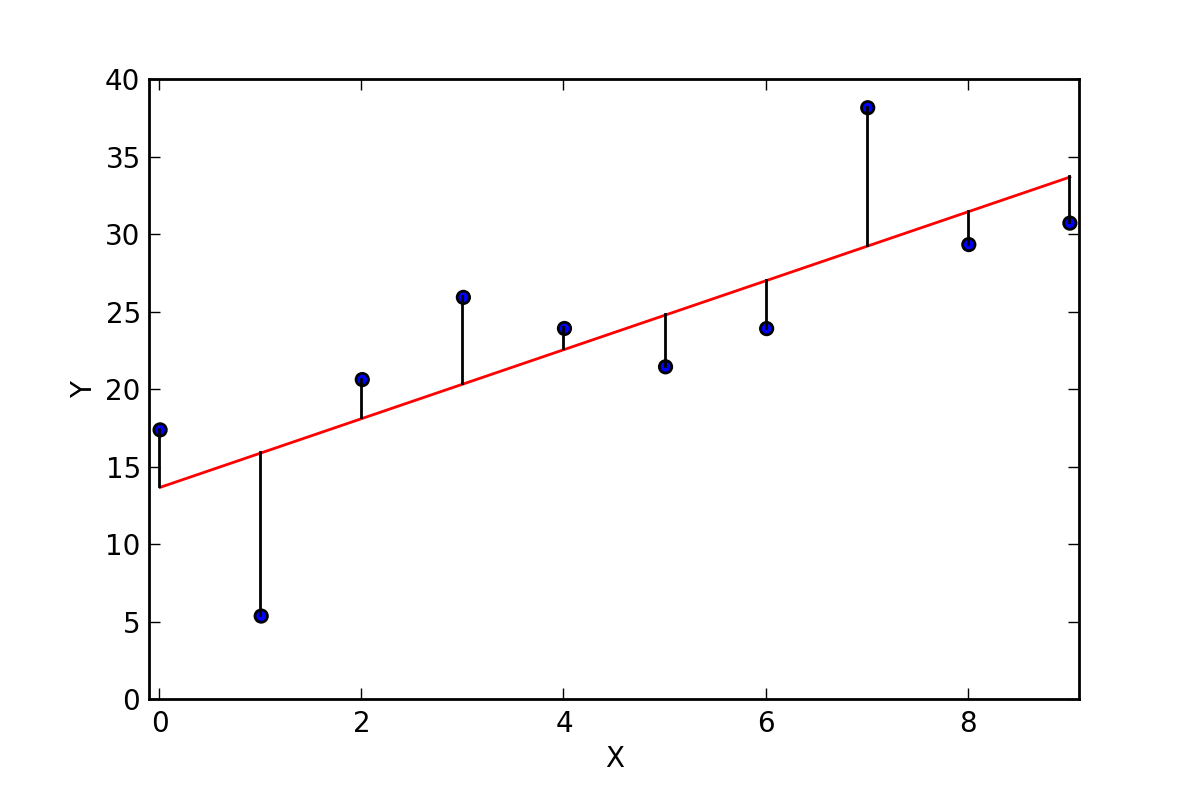
\includegraphics[width=0.5\textwidth]{MAE.png} 
    \end{figure}
    \[
    J(w) = \sum_{i=1}^{n} \left( y^{(i)} - h_w(x^{(i)}) \right)^2 = \sum_{i=1}^{n} \left( y^{(i)} - w_0 - w_1 x^{(i)} \right)^2
    \]
\end{frame}

\begin{frame}{Cost Function Optimization}
    \item The goal of linear regression is to minimize the sum of squared errors (SSE) between the predicted values and the actual values.
    
    \begin{equation}
    J(w) = \sum_{i=1}^{n} \left( y^{(i)} - w_0 - w_1 x^{(i)} \right)^2
    \end{equation}
\end{frame}

\begin{frame}{Condition For Optimal Value}
    \item To find the optimal values of $w_0$ and $w_1$, we need to solve the following partial derivatives and set them to zero:
    \begin{equation}
    \frac{\partial J(w)}{\partial w_0} = 0
    \end{equation}

    \begin{equation}
    \frac{\partial J(w)}{\partial w_1} = 0
    \end{equation}
\end{frame}

\begin{frame}{Optimization}
    \begin{figure}[h]
        \centering
        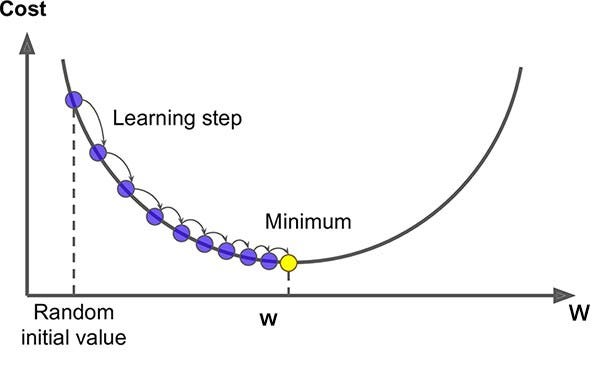
\includegraphics[width=0.5\textwidth]{OptReg.jpg} 
    \end{figure}
\end{frame}

\section{Linear Regression}
\begin{frame}{What is Regression?}
\textbf{Regression} is a statistical method used to model the relationship between a dependent variable (output) and one or more independent variables (inputs). The goal is to predict the output based on input features.

\vspace{0.5cm}
\textbf{Linear Regression} is a type of regression where the relationship between variables is modeled as a straight line. The formula is:
\begin{equation}
Y = w_0 + w_1 X
\end{equation}
Where:
\begin{itemize}
    \item $Y$: Predicted value (dependent variable)
    \item $X$: Input feature (independent variable)
    \item $w_0$: Intercept (bias term)
    \item $w_1$: Slope (weight)
\end{itemize}
\end{frame}

\begin{frame}{Common Example: Predicting House Prices}
\textbf{Problem:} A real estate agent wants to predict the price of a house based on its size.

\textbf{Given Data:}
\begin{center}
\begin{tabular}{|c|c|}
\hline
Size (sq ft) & Price (USD) \\
\hline
1000 & 200,000 \\
1500 & 300,000 \\
2000 & 400,000 \\
2500 & 500,000 \\
\hline
\end{tabular}
\end{center}

\textbf{Solution:} Using linear regression, we fit the line:
\begin{equation}
Y = w_0 + w_1 X
\end{equation}
\textbf{Steps:}
\begin{itemize}
    \item Calculate $w_1$ (slope): $w_1 = \frac{\sum (X - \bar{X})(Y - \bar{Y})}{\sum (X - \bar{X})^2}$
    \item Calculate $w_0$ (intercept): $w_0 = \bar{Y} - w_1 \bar{X}$
\end{itemize}
\end{frame}

\begin{frame}{Medical Example: Predicting Blood Pressure}
\textbf{Problem:} A doctor wants to predict a patient's systolic blood pressure based on their age.

\textbf{Given Data:}
\begin{center}
\begin{tabular}{|c|c|}
\hline
Age (years) & Blood Pressure (mmHg) \\
\hline
30 & 120 \\
40 & 130 \\
50 & 140 \\
60 & 150 \\
\hline
\end{tabular}
\end{center}

\textbf{Solution:} Using linear regression, we fit the line:
\begin{equation}
Y = w_0 + w_1 X
\end{equation}
\textbf{Steps:}
\begin{itemize}
    \item Calculate $w_1$ (slope): $w_1 = \frac{\sum (X - \bar{X})(Y - \bar{Y})}{\sum (X - \bar{X})^2}$
    \item Calculate $w_0$ (intercept): $w_0 = \bar{Y} - w_1 \bar{X}$
\end{itemize}
\end{frame}

\begin{frame}{House Price Prediction Plot}
    \begin{figure}[h]
        \centering
        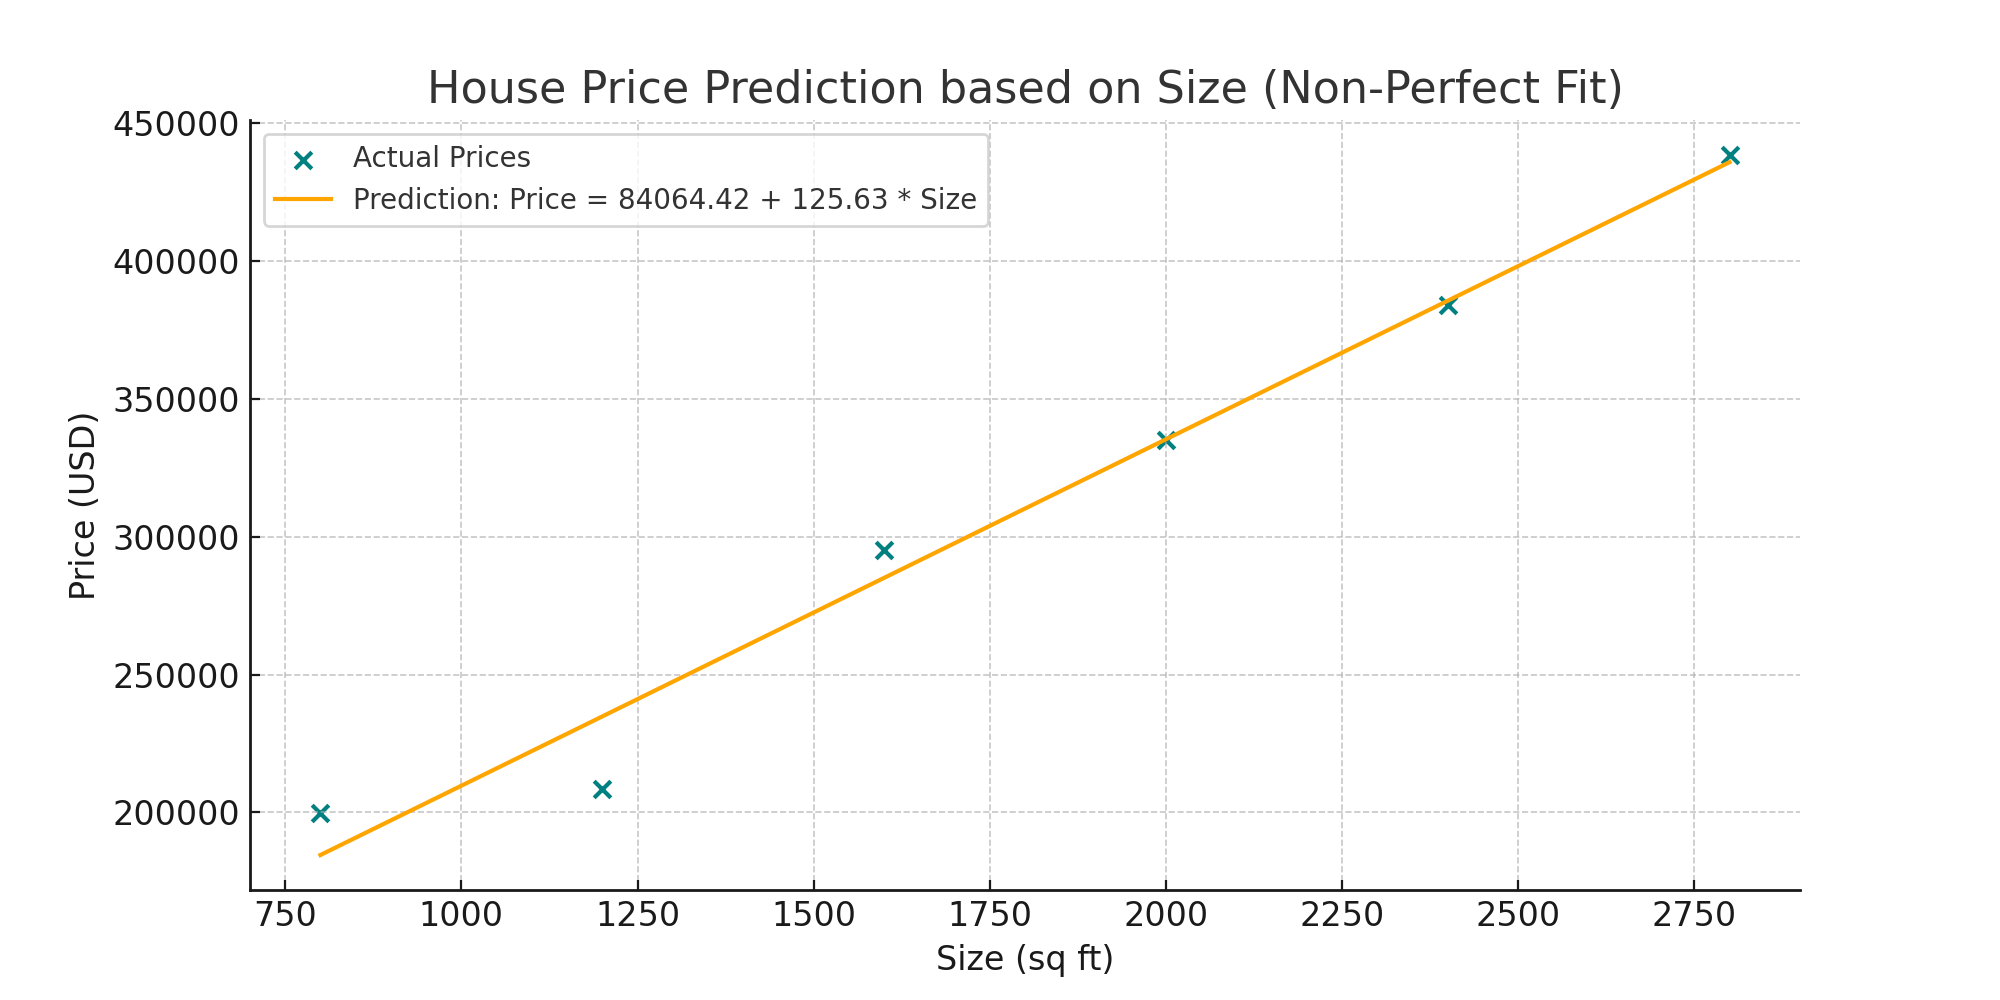
\includegraphics[width=0.5\textwidth]{house_price_non_perfect_plot.png} 
    \end{figure}
\end{frame}

\section{Polynomial Regression}

\begin{frame}{What is Polynomial Regression?}
\textbf{Polynomial Regression} is an extension of linear regression where the relationship between the independent variable $X$ and the dependent variable $Y$ is modeled as an $n^{th}$ degree polynomial.

\vspace{0.5cm}
The formula for polynomial regression is:
\begin{equation}
Y = w_0 + w_1 X + w_2 X^2 + \cdots + w_n X^n
\end{equation}
Where:
\begin{itemize}
    \item $Y$: Predicted value (dependent variable)
    \item $X$: Input feature (independent variable)
    \item $w_0, w_1, \dots, w_n$: Coefficients to be learned
\end{itemize}
\textbf{Why use Polynomial Regression?}
\begin{itemize}
    \item To capture non-linear relationships in the data.
    \item Linear regression fails to fit curves, while polynomial regression can.
\end{itemize}
\end{frame}

\begin{frame}{Example: Predicting Tumor Growth}
\textbf{Problem:} A researcher wants to model the relationship between time (days) and the size of a tumor (in cm).

\textbf{Given Data:}
\begin{center}
\begin{tabular}{|c|c|}
\hline
Time (days) & Tumor Size (cm) \\
\hline
1 & 2.1 \\
2 & 4.5 \\
3 & 8.0 \\
4 & 14.2 \\
5 & 23.5 \\
6 & 35.8 \\
\hline
\end{tabular}
\end{center}
\end{frame}

\begin{frame}{Solution Steps}
\item Using polynomial regression, we fit a curve:
\begin{equation}
Y = w_0 + w_1 X + w_2 X^2
\end{equation}
\textbf{Steps:}
\begin{itemize}
    \item Calculate coefficients $w_0$, $w_1$, $w_2$ using least squares method.
    \item Plot the curve and observe the fit.
\end{itemize}
\textbf{Result:} The model captures the non-linear growth pattern of the tumor.
\end{frame}

\begin{frame}{Polynomial Regression Plot}
    \begin{figure}[h]
        \centering
        \includegraphics[width=0.5\textwidth]{polynomialregression.png} 
    \end{figure}
\end{frame}

\begin{frame}{Why Polynomial?}
    \begin{figure}[h]
        \centering
        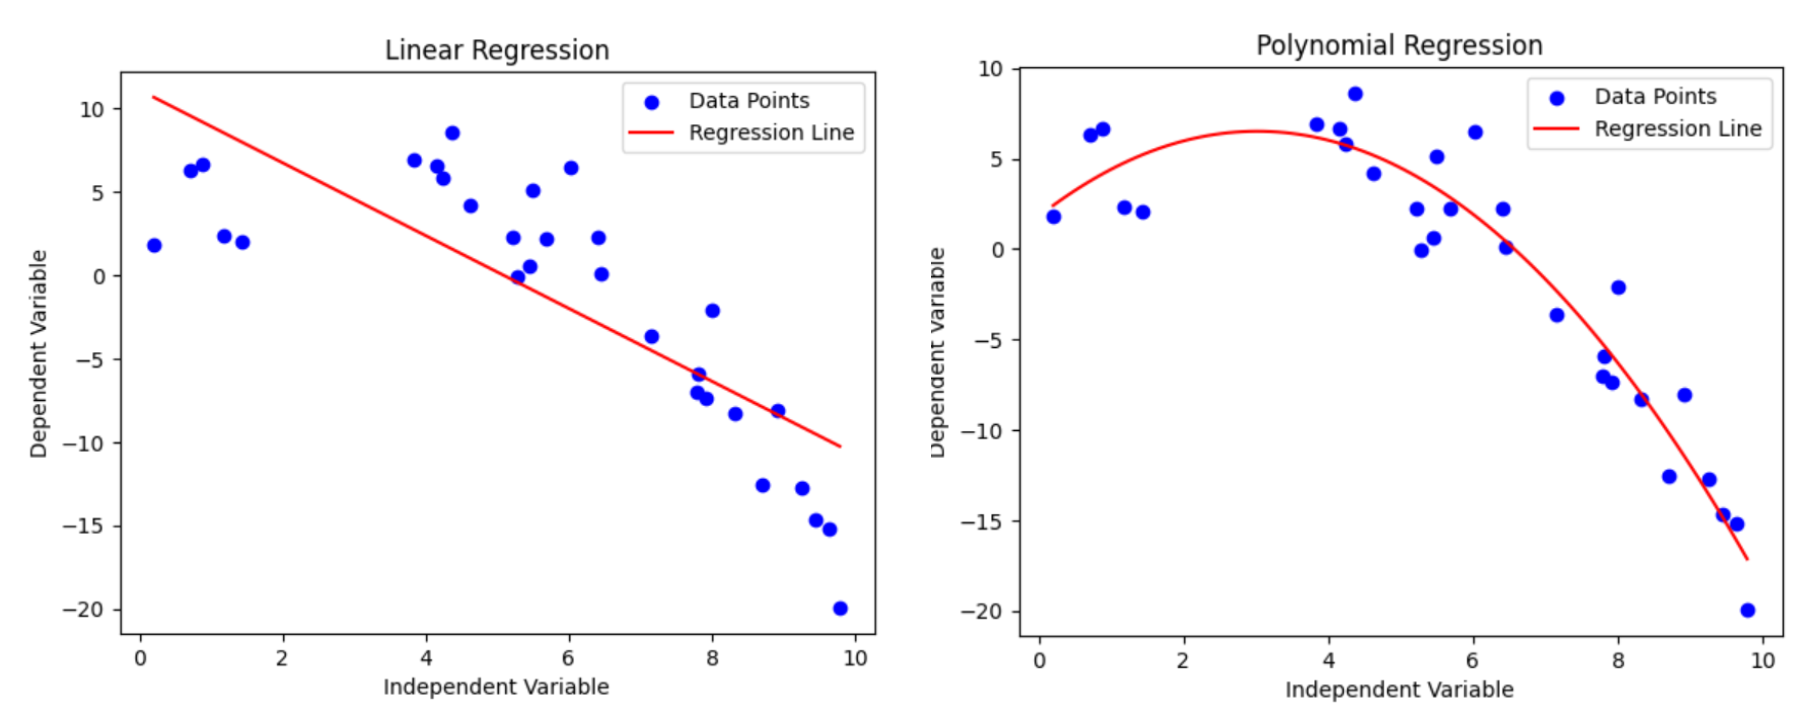
\includegraphics[width=0.5\textwidth]{PolynomialVsLinear.png} 
    \end{figure}
\end{frame}

\section{Evaluation}
\begin{frame}{What is Evaluation?}
    \item Evaluation in machine learning is the process of measuring how well a model performs on a given task. It helps to:
\begin{itemize}
    \item Assess model accuracy.
    \item Identify overfitting or underfitting.
    \item Compare different models.
\end{itemize}
\end{frame}

\begin{frame}{Why Choose the Right Metric?}
    \begin{itemize}
        \item Different tasks (regression, classification) require different evaluation methods.
        \item Incorrect metrics can lead to wrong conclusions.
        \item Metrics must align with business goals and data characteristics.
    \end{itemize}
\end{frame}

\begin{frame}{Mean Absolute Error (MAE)}
\textbf{Formula:}
\begin{equation}
MAE = \frac{1}{n} \sum_{i=1}^{n} |y_i - \hat{y}_i|
\end{equation}
\textbf{When to Use:}
\begin{itemize}
    \item When you want to measure the average magnitude of errors.
    \item Suitable when all errors have the same importance.
\end{itemize}
\textbf{Pros:} Easy to interpret.
\textbf{Cons:} Less sensitive to large errors.
\end{frame}

\begin{frame}{Mean Squared Error (MSE)}
\textbf{Formula:}
\begin{equation}
MSE = \frac{1}{n} \sum_{i=1}^{n} (y_i - \hat{y}_i)^2
\end{equation}
\textbf{When to Use:}
\begin{itemize}
    \item When you want to penalize larger errors more.
    \item Common in regression problems.
\end{itemize}
\textbf{Pros:} Penalizes large errors more than MAE.
\textbf{Cons:} Sensitive to outliers.
\end{frame}

\begin{frame}{Root Mean Squared Error (RMSE)}
\textbf{Formula:}
\begin{equation}
RMSE = \sqrt{\frac{1}{n} \sum_{i=1}^{n} (y_i - \hat{y}_i)^2}
\end{equation}
\textbf{When to Use:}
\begin{itemize}
    \item When you want to interpret the error in the same unit as the target variable.
    \item Useful for comparing models.
\end{itemize}
\textbf{Pros:} Easy to interpret.
\textbf{Cons:} Sensitive to outliers.
\end{frame}

\begin{frame}{R-Squared ($R^2$)}
\textbf{Formula:}
\begin{equation}
R^2 = 1 - \frac{\sum_{i=1}^{n} (y_i - \hat{y}_i)^2}{\sum_{i=1}^{n} (y_i - \bar{y})^2}
\end{equation}
\textbf{When to Use:}
\begin{itemize}
    \item To measure how well the model explains the variance in the data.
    \item Useful for determining model fit.
\end{itemize}
\textbf{Pros:} Provides a normalized score.
\textbf{Cons:} Can be misleading for non-linear models.
\end{frame}

\begin{frame}{Summary of Evaluation Metrics}
\begin{table}[]
\centering
\begin{tabular}{|c|c|c|}
\hline
\textbf{Metric} & \textbf{Formula} & \textbf{When to Use} \\
\hline
MAE & $\frac{1}{n} \sum |y_i - \hat{y}_i|$ & Average magnitude of errors \\
MSE & $\frac{1}{n} \sum (y_i - \hat{y}_i)^2$ & Penalizes larger errors more \\
RMSE & $\sqrt{\frac{1}{n} \sum (y_i - \hat{y}_i)^2}$ & Same unit as target variable \\
$R^2$ & $1 - \frac{\sum (y_i - \hat{y}_i)^2}{\sum (y_i - \bar{y})^2}$ & Explains variance in the data \\
\hline
\end{tabular}
\end{table}
\end{frame}

\section{Generalization & Regularization}
\begin{frame}{What is Generalization?}
\textbf{Generalization} in machine learning refers to a model's ability to perform well on unseen data that it has not encountered during training. It is a measure of how well the model can apply the knowledge learned from the training data to new, real-world scenarios.

\vspace{0.5cm}
\textbf{Key Concepts:}
\begin{itemize}
    \item \textbf{Training Error:} The error a model makes on the training data.
    \item \textbf{Test Error:} The error a model makes on unseen data.
    \item \textbf{Overfitting:} When a model performs well on training data but poorly on test data.
    \item \textbf{Underfitting:} When a model performs poorly on both training and test data.
\end{itemize}
\end{frame}

\begin{frame}{Why is Generalization Important?}
\begin{itemize}
    \item A well-generalized model can make accurate predictions on new, unseen data.
    \item It ensures that the model is not just memorizing the training data but learning patterns that apply broadly.
    \item Poor generalization leads to models that either overfit or underfit the data, resulting in poor performance in real-world applications.
\end{itemize}

\textbf{Example:} A model trained to predict house prices should perform well not only on the training dataset but also on new properties it hasn't seen before.
\end{frame}

\begin{frame}{Overfitting vs. Underfitting}
\textbf{Overfitting:}
\begin{itemize}
    \item Model captures noise and irrelevant details in the training data.
    \item High training accuracy but poor test accuracy.
    \item Solution: Regularization, pruning, cross-validation.
\end{itemize}


\textbf{Underfitting:}
\begin{itemize}
    \item Model fails to capture the underlying pattern in the data.
    \item Both training and test accuracy are low.
    \item Solution: Use a more complex model, feature engineering.
\end{itemize}
\end{frame}

\begin{frame}{How to Improve Generalization?}
\begin{itemize}
    \item \textbf{Cross-Validation:} Split the dataset into multiple folds and validate the model on different subsets.
    \item \textbf{Regularization:} Add a penalty term to the loss function to prevent the model from becoming too complex.
    \item \textbf{Early Stopping:} Stop training when the performance on a validation set stops improving.
    \item \textbf{Data Augmentation:} Increase the diversity of the training data by creating variations of the existing data.
    \item \textbf{Dropout:} Randomly drop units in a neural network during training to prevent overfitting.
\end{itemize}
\end{frame}

\begin{frame}{Variance & Bias}
    \begin{figure}[h]
        \centering
        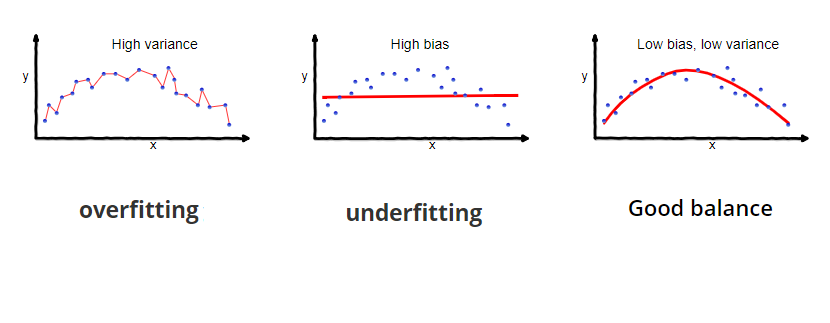
\includegraphics[width=0.7\textwidth]{BiasVariance.png} 
    \end{figure}
\end{frame}

\begin{frame}{What is Regularization?}
\textbf{Regularization} is a technique used in regression models to reduce overfitting by adding a penalty term to the model's loss function. It prevents the model from becoming too complex and helps improve generalization to unseen data.

\vspace{0.5cm}
\textbf{Why Use Regularization?}
\begin{itemize}
    \item To prevent overfitting.
    \item To ensure the model performs well on both training and test data.
    \item To improve model interpretability by reducing overly complex solutions.
\end{itemize}
\end{frame}

\begin{frame}{Regularized Linear Regression Formula}
The objective in linear regression is to minimize the cost function:
\begin{equation}
J(w) = \sum_{i=1}^{n} \left( y^{(i)} - \left( w_0 + w_1 x^{(i)} \right) \right)^2
\end{equation}

In regularized regression, a penalty term is added to the cost function to prevent large coefficient values:
\begin{equation}
J(w) = \sum_{i=1}^{n} \left( y^{(i)} - \left( w_0 + w_1 x^{(i)} \right) \right)^2 + \lambda R(w)
\end{equation}
where:
\begin{itemize}
    \item $\lambda$ is the regularization parameter.
    \item $R(w)$ is the regularization term.
\end{itemize}
\end{frame}

\begin{frame}{Types of Regularization}
There are two main types of regularization used in regression:
\begin{itemize}
    \item \textbf{L1 Regularization (Lasso)}
    \item \textbf{L2 Regularization (Ridge)}
\end{itemize}
Both add a penalty term to the cost function, but they do so in different ways.
\end{frame}

\begin{frame}{L1 Regularization (Lasso)}
L1 regularization adds the sum of the absolute values of the coefficients to the cost function:
\begin{equation}
J(w) = \sum_{i=1}^{n} \left( y^{(i)} - \hat{y}^{(i)} \right)^2 + \lambda \sum_{j=1}^{p} |w_j|
\end{equation}

\textbf{Effect:} Encourages sparsity by shrinking some coefficients to exactly zero, effectively performing feature selection.
\end{frame}

\begin{frame}{L2 Regularization (Ridge)}
L2 regularization adds the sum of the squared values of the coefficients to the cost function:
\begin{equation}
J(w) = \sum_{i=1}^{n} \left( y^{(i)} - \hat{y}^{(i)} \right)^2 + \lambda \sum_{j=1}^{p} w_j^2
\end{equation}

\textbf{Effect:} Prevents large coefficients by penalizing their magnitude, but does not reduce them to zero.
\end{frame}



\begin{frame}
    \begin{center}
        {\Huge\ \color{red}For more information and code check the related notebook}
    \end{center}
\end{frame}


\begin{frame}
    \begin{center}
        {\Huge\ End of Regression}
    \end{center}
\end{frame}

\end{document}

